\documentclass{article}%
\usepackage[T1]{fontenc}%
\usepackage[utf8]{inputenc}%
\usepackage{lmodern}%
\usepackage{textcomp}%
\usepackage{lastpage}%
\usepackage{authblk}%
\usepackage{graphicx}%
%
\title{Signaling pathway underlying the up{-}regulatory effect of TNF{-}a on the Na+/K+ ATPase in HepG2 cells}%
\author{Zachary Benson}%
\affil{Department of Pathophysiology, School of Pharmacy and Biochemistry, University of Buenos Aires, INFIBIOC{-}CONICET, Argentina}%
\date{01{-}01{-}2001}%
%
\begin{document}%
\normalsize%
\maketitle%
\section{Abstract}%
\label{sec:Abstract}%
Scientists at the University of Southern California (USC) have shown that a transgenic mouse and which may one day replace chemical therapies for cattle infected with mycobacterium tuberculosis, a bacterial lung disease, activated the subunit of the mycobacterium mycobacteria that infects many animals, not just cattle.\newline%
USC's researchers demonstrated that leukotoxin activity in cattle (Icobacterium:NBM1) is proportional to the amount of curative agents available in the treatable lung disease form of the mycobacterium disease. This study, reported today in the journal Nature Genetics, adds new details to our understanding of how transgenic mice attack bacteria.\newline%
According to Matt Mead, a professor of pathology and immunology at USC and one of the researchers on the study, the results may prove useful in the development of a new therapeutic strategy to treat cattle infected with TB.\newline%
"Using transgenic mice to battle TB might prove to be more effective than conventional therapy in fighting the disease and may be more efficient and cost{-}effective than treatments using toxins that interact with bacteria naturally," said Mead. "Because TB is actually a bacterial disease and not a virus, we hoped that the conduct of mutant protease activity would indirectly translate into antiviral activity. Previous studies have shown that a molecular signature in TB bacteria is generated in a specific cell."\newline%
"By providing a different target by mutation to the disease's killer bacterium, transgenic mice may be considered an example of a novel anti{-}TB therapy," he said.\newline%
The transgenic mouse, which has been transferred to the Queensland University of Technology (QUT) laboratory in the United States, was created with human experimental leukotivosis bacteria that were homologous with the mycobacterium mycobacteria found in cattle. That means the agents that the cattle carried were the same as the ones that the cattle carried to the United States. However, the mutant bacteria had a different transgenesis signature, a pattern of abnormalities in cellular anatomy that could raise the transgenic mouse's growth hormone, which contributed to the growth of the animal's intestinal cells.\newline%
A significant caveat to using transgenic mice in cancer and other serious diseases has been that the animals would be treated either with a probiotic or antibiotics. But in certain clinical trials using transgenic mice in various cancer settings, the probiotics were perceived as both safe and effective in treating the cancer. The scientists had not yet determined if the mutant bacteria has the same degree of a range or tolerance for nonreactive antibiotics as normal bacteria, so transgenic mice may not be an indication of effective antibiotics.\newline%
USC researchers examined 64 lung infected cattle, and found that transgenic mice showed a higher degree of response to antibiotics than non{-}mutated cattle. But the similarities went beyond bacterial activity. Dr. Mark Cordey, chief of the Laboratory of Infectious Diseases at QUT and the lead author of the study, and PhD candidate Elizabeth Wadhwa said they were able to differentiate respiratory matter from the bacterium germ codes, especially the B{-}rhoin1 mycobacterium.\newline%
"This study provides evidence that transgenic mice can protect both animals and humans against tuberculosis," said Cordey. "It may be that the mycobacterium disease could be treated with a transgenic aid in lung sanitation. But the most important thing is that they have the ability to create a functional disease like tuberculosis.

%
\subsection{Image Analysis}%
\label{subsec:ImageAnalysis}%


\begin{figure}[h!]%
\centering%
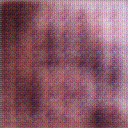
\includegraphics[width=150px]{500_fake_images/samples_5_82.png}%
\caption{A Black And White Photo Of A Black And White Photo}%
\end{figure}

%
\end{document}